\documentclass[]{article}
\usepackage{lmodern}
\usepackage{amssymb,amsmath}
\usepackage{ifxetex,ifluatex}
\usepackage{fixltx2e} % provides \textsubscript
\ifnum 0\ifxetex 1\fi\ifluatex 1\fi=0 % if pdftex
  \usepackage[T1]{fontenc}
  \usepackage[utf8]{inputenc}
\else % if luatex or xelatex
  \ifxetex
    \usepackage{mathspec}
  \else
    \usepackage{fontspec}
  \fi
  \defaultfontfeatures{Ligatures=TeX,Scale=MatchLowercase}
\fi
% use upquote if available, for straight quotes in verbatim environments
\IfFileExists{upquote.sty}{\usepackage{upquote}}{}
% use microtype if available
\IfFileExists{microtype.sty}{%
\usepackage{microtype}
\UseMicrotypeSet[protrusion]{basicmath} % disable protrusion for tt fonts
}{}
\usepackage[margin=1in]{geometry}
\usepackage{hyperref}
\hypersetup{unicode=true,
            pdftitle={NZ GREEN Grid Household Power Demand Profiles: Hot Water},
            pdfauthor={Ben Anderson (b.anderson@soton.ac.uk, @dataknut)},
            pdfborder={0 0 0},
            breaklinks=true}
\urlstyle{same}  % don't use monospace font for urls
\usepackage{color}
\usepackage{fancyvrb}
\newcommand{\VerbBar}{|}
\newcommand{\VERB}{\Verb[commandchars=\\\{\}]}
\DefineVerbatimEnvironment{Highlighting}{Verbatim}{commandchars=\\\{\}}
% Add ',fontsize=\small' for more characters per line
\usepackage{framed}
\definecolor{shadecolor}{RGB}{248,248,248}
\newenvironment{Shaded}{\begin{snugshade}}{\end{snugshade}}
\newcommand{\KeywordTok}[1]{\textcolor[rgb]{0.13,0.29,0.53}{\textbf{#1}}}
\newcommand{\DataTypeTok}[1]{\textcolor[rgb]{0.13,0.29,0.53}{#1}}
\newcommand{\DecValTok}[1]{\textcolor[rgb]{0.00,0.00,0.81}{#1}}
\newcommand{\BaseNTok}[1]{\textcolor[rgb]{0.00,0.00,0.81}{#1}}
\newcommand{\FloatTok}[1]{\textcolor[rgb]{0.00,0.00,0.81}{#1}}
\newcommand{\ConstantTok}[1]{\textcolor[rgb]{0.00,0.00,0.00}{#1}}
\newcommand{\CharTok}[1]{\textcolor[rgb]{0.31,0.60,0.02}{#1}}
\newcommand{\SpecialCharTok}[1]{\textcolor[rgb]{0.00,0.00,0.00}{#1}}
\newcommand{\StringTok}[1]{\textcolor[rgb]{0.31,0.60,0.02}{#1}}
\newcommand{\VerbatimStringTok}[1]{\textcolor[rgb]{0.31,0.60,0.02}{#1}}
\newcommand{\SpecialStringTok}[1]{\textcolor[rgb]{0.31,0.60,0.02}{#1}}
\newcommand{\ImportTok}[1]{#1}
\newcommand{\CommentTok}[1]{\textcolor[rgb]{0.56,0.35,0.01}{\textit{#1}}}
\newcommand{\DocumentationTok}[1]{\textcolor[rgb]{0.56,0.35,0.01}{\textbf{\textit{#1}}}}
\newcommand{\AnnotationTok}[1]{\textcolor[rgb]{0.56,0.35,0.01}{\textbf{\textit{#1}}}}
\newcommand{\CommentVarTok}[1]{\textcolor[rgb]{0.56,0.35,0.01}{\textbf{\textit{#1}}}}
\newcommand{\OtherTok}[1]{\textcolor[rgb]{0.56,0.35,0.01}{#1}}
\newcommand{\FunctionTok}[1]{\textcolor[rgb]{0.00,0.00,0.00}{#1}}
\newcommand{\VariableTok}[1]{\textcolor[rgb]{0.00,0.00,0.00}{#1}}
\newcommand{\ControlFlowTok}[1]{\textcolor[rgb]{0.13,0.29,0.53}{\textbf{#1}}}
\newcommand{\OperatorTok}[1]{\textcolor[rgb]{0.81,0.36,0.00}{\textbf{#1}}}
\newcommand{\BuiltInTok}[1]{#1}
\newcommand{\ExtensionTok}[1]{#1}
\newcommand{\PreprocessorTok}[1]{\textcolor[rgb]{0.56,0.35,0.01}{\textit{#1}}}
\newcommand{\AttributeTok}[1]{\textcolor[rgb]{0.77,0.63,0.00}{#1}}
\newcommand{\RegionMarkerTok}[1]{#1}
\newcommand{\InformationTok}[1]{\textcolor[rgb]{0.56,0.35,0.01}{\textbf{\textit{#1}}}}
\newcommand{\WarningTok}[1]{\textcolor[rgb]{0.56,0.35,0.01}{\textbf{\textit{#1}}}}
\newcommand{\AlertTok}[1]{\textcolor[rgb]{0.94,0.16,0.16}{#1}}
\newcommand{\ErrorTok}[1]{\textcolor[rgb]{0.64,0.00,0.00}{\textbf{#1}}}
\newcommand{\NormalTok}[1]{#1}
\usepackage{longtable,booktabs}
\usepackage{graphicx,grffile}
\makeatletter
\def\maxwidth{\ifdim\Gin@nat@width>\linewidth\linewidth\else\Gin@nat@width\fi}
\def\maxheight{\ifdim\Gin@nat@height>\textheight\textheight\else\Gin@nat@height\fi}
\makeatother
% Scale images if necessary, so that they will not overflow the page
% margins by default, and it is still possible to overwrite the defaults
% using explicit options in \includegraphics[width, height, ...]{}
\setkeys{Gin}{width=\maxwidth,height=\maxheight,keepaspectratio}
\IfFileExists{parskip.sty}{%
\usepackage{parskip}
}{% else
\setlength{\parindent}{0pt}
\setlength{\parskip}{6pt plus 2pt minus 1pt}
}
\setlength{\emergencystretch}{3em}  % prevent overfull lines
\providecommand{\tightlist}{%
  \setlength{\itemsep}{0pt}\setlength{\parskip}{0pt}}
\setcounter{secnumdepth}{5}
% Redefines (sub)paragraphs to behave more like sections
\ifx\paragraph\undefined\else
\let\oldparagraph\paragraph
\renewcommand{\paragraph}[1]{\oldparagraph{#1}\mbox{}}
\fi
\ifx\subparagraph\undefined\else
\let\oldsubparagraph\subparagraph
\renewcommand{\subparagraph}[1]{\oldsubparagraph{#1}\mbox{}}
\fi

%%% Use protect on footnotes to avoid problems with footnotes in titles
\let\rmarkdownfootnote\footnote%
\def\footnote{\protect\rmarkdownfootnote}

%%% Change title format to be more compact
\usepackage{titling}

% Create subtitle command for use in maketitle
\newcommand{\subtitle}[1]{
  \posttitle{
    \begin{center}\large#1\end{center}
    }
}

\setlength{\droptitle}{-2em}

  \title{NZ GREEN Grid Household Power Demand Profiles: Hot Water}
    \pretitle{\vspace{\droptitle}\centering\huge}
  \posttitle{\par}
  \subtitle{Data extraction and preliminary plots}
  \author{Ben Anderson
(\href{mailto:b.anderson@soton.ac.uk}{\nolinkurl{b.anderson@soton.ac.uk}},
\texttt{@dataknut})}
    \preauthor{\centering\large\emph}
  \postauthor{\par}
      \predate{\centering\large\emph}
  \postdate{\par}
    \date{Last run at: 2018-07-26 17:40:22}


\begin{document}
\maketitle

{
\setcounter{tocdepth}{2}
\tableofcontents
}
\newpage

\section{Status}\label{status}

Full run using all data from /Volumes/hum-csafe/Research Projects/GREEN
Grid/\_RAW DATA/GridSpyData/

\section{Citation}\label{citation}

If you wish to use any of the material from this report please cite as:

\begin{itemize}
\tightlist
\item
  Anderson, B. (2018) GREEN Grid Heat Pump Profiles, University of
  Otago: Dunedin, NZ.
\end{itemize}

\newpage

\section{Introduction}\label{introduction}

Report circulation:

\begin{itemize}
\tightlist
\item
  Restricted to:
  \href{https://www.otago.ac.nz/centre-sustainability/research/energy/otago050285.html}{NZ
  GREEN Grid} project partners and contractors.
\end{itemize}

\subsection{Purpose}\label{purpose}

This report is intended to:

\begin{itemize}
\tightlist
\item
  load and clean the project electricity power data (Grid Spy)
\item
  select the Heat Pump circuits (via their labels)
\item
  build exploratory demand profiles
\end{itemize}

\subsection{Requirements:}\label{requirements}

\begin{itemize}
\tightlist
\item
  cleaned and safe grid spy 1 minute data processed via
  \url{https://git.soton.ac.uk/ba1e12/nzGREENGrid/blob/master/dataProcessing/processNZGGElecCons1minData.Rmd}
\end{itemize}

\subsection{History}\label{history}

Generally tracked via our git.soton
\href{https://git.soton.ac.uk/ba1e12/nzGREENGrid}{repo}:

\begin{itemize}
\tightlist
\item
  \href{https://git.soton.ac.uk/ba1e12/nzGREENGrid/commits/master}{history}
\item
  \href{https://git.soton.ac.uk/ba1e12/nzGREENGrid/issues}{issues}
\end{itemize}

\subsection{Support}\label{support}

This work was supported by:

\begin{itemize}
\tightlist
\item
  The \href{https://www.otago.ac.nz/}{University of Otago}
\item
  The New Zealand \href{http://www.mbie.govt.nz/}{Ministry of Business,
  Innovation and Employment (MBIE)}
\item
  \href{http://www.energy.soton.ac.uk/tag/spatialec/}{SPATIALEC} - a
  \href{http://ec.europa.eu/research/mariecurieactions/about-msca/actions/if/index_en.htm}{Marie
  Skłodowska-Curie Global Fellowship} based at the University of Otago's
  \href{http://www.otago.ac.nz/centre-sustainability/staff/otago673896.html}{Centre
  for Sustainability} (2017-2019) \& the University of Southampton's
  Sustainable Energy Research Group (2019-202).
\end{itemize}

This work is (c) 2018 the University of Southampton.

We do not `support' the code but if you have a problem check the
\href{https://git.soton.ac.uk/ba1e12/nzGREENGrid/issues}{issues} on our
\href{https://git.soton.ac.uk/ba1e12/nzGREENGrid}{repo} and if it
doesn't already exist, open one. We might be able to fix it :-)

\section{Load data files}\label{load-data-files}

\subsection{Grid Spy metadata}\label{grid-spy-metadata}

In this section we load metadata from /Users/ben/Syncplicity
Folders/Green Grid Project Management Folder/Gridspy/Master list of
Gridspy units.xlsx to link to the power data.

\begin{longtable}[]{@{}lllllll@{}}
\toprule
sample & hhID & Adults & Teenagers & Children & removed &
nAdults\tabularnewline
\midrule
\endhead
Powerco & rf\_06 & 2 & NA & NA & NA & 2\tabularnewline
Powerco & rf\_07 & 2 & NA & 2 & NA & 2\tabularnewline
Powerco & rf\_08 & 2 & NA & NA & NA & 2\tabularnewline
Powerco & rf\_09 & 2 & NA & 1 & 42171 & 2\tabularnewline
Powerco & rf\_10 & 2 & NA & 1(3yo) & NA & 3\tabularnewline
Powerco & rf\_11 & NA & NA & NA & NA & 1\tabularnewline
\bottomrule
\end{longtable}

\subsection{Grid Spy data}\label{grid-spy-data}

In this section we load the cleaned data files from
/Volumes/hum-csafe/Research Projects/GREEN
Grid/Clean\_data/safe/gridSpy/1min/data/. If we loaded all the data at
once and then filtered out what we want we might run out of memory so we
filter as we load. Set the filters here:

\begin{Shaded}
\begin{Highlighting}[]
\NormalTok{circuitPattern <-}\StringTok{ }\NormalTok{params}\OperatorTok{$}\NormalTok{circuitPattern}
\NormalTok{dateFrom <-}\StringTok{ }\NormalTok{params}\OperatorTok{$}\NormalTok{dateFrom}
\NormalTok{dateTo <-}\StringTok{ }\NormalTok{params}\OperatorTok{$}\NormalTok{dateTo}

\NormalTok{plotCaption <-}\StringTok{ }\KeywordTok{paste0}\NormalTok{(}\StringTok{"Source: "}\NormalTok{, fpath,}
                      \StringTok{"}\CharTok{\textbackslash{}n}\StringTok{Circuits: "}\NormalTok{, circuitPattern, }\StringTok{" from "}\NormalTok{, dateFrom, }\StringTok{" to "}\NormalTok{, dateTo)}
\end{Highlighting}
\end{Shaded}

So we are looking for Hot Water circuits between 2015-04-01 and
2016-03-31. We do this by checking to see if the extract file has
already been created. If so we load it. If not, we create it.

Loading: /Volumes/hum-csafe/Research Projects/GREEN
Grid/Clean\_data/safe/gridSpy/1min/dataExtracts/Hot
Water\_2015-04-01\_2016-03-31\_observations.csv.gz (needs to exist!)

The following table summarises the Hot Water data we have found.

\begin{longtable}[]{@{}llllll@{}}
\toprule
\begin{minipage}[b]{0.03\columnwidth}\raggedright\strut
\strut
\end{minipage} & \begin{minipage}[b]{0.15\columnwidth}\raggedright\strut
hhID\strut
\end{minipage} & \begin{minipage}[b]{0.24\columnwidth}\raggedright\strut
r\_dateTime\strut
\end{minipage} & \begin{minipage}[b]{0.15\columnwidth}\raggedright\strut
circuitLabel\strut
\end{minipage} & \begin{minipage}[b]{0.12\columnwidth}\raggedright\strut
circuitID\strut
\end{minipage} & \begin{minipage}[b]{0.14\columnwidth}\raggedright\strut
powerW\strut
\end{minipage}\tabularnewline
\midrule
\endhead
\begin{minipage}[t]{0.03\columnwidth}\raggedright\strut
\strut
\end{minipage} & \begin{minipage}[t]{0.15\columnwidth}\raggedright\strut
Length:14493877\strut
\end{minipage} & \begin{minipage}[t]{0.24\columnwidth}\raggedright\strut
Min. :2015-04-01 00:00:00\strut
\end{minipage} & \begin{minipage}[t]{0.15\columnwidth}\raggedright\strut
Length:14493877\strut
\end{minipage} & \begin{minipage}[t]{0.12\columnwidth}\raggedright\strut
Min. :1574\strut
\end{minipage} & \begin{minipage}[t]{0.14\columnwidth}\raggedright\strut
Min. :-1110.0\strut
\end{minipage}\tabularnewline
\begin{minipage}[t]{0.03\columnwidth}\raggedright\strut
\strut
\end{minipage} & \begin{minipage}[t]{0.15\columnwidth}\raggedright\strut
Class :character\strut
\end{minipage} & \begin{minipage}[t]{0.24\columnwidth}\raggedright\strut
1st Qu.:2015-06-22 16:46:00\strut
\end{minipage} & \begin{minipage}[t]{0.15\columnwidth}\raggedright\strut
Class :character\strut
\end{minipage} & \begin{minipage}[t]{0.12\columnwidth}\raggedright\strut
1st Qu.:2248\strut
\end{minipage} & \begin{minipage}[t]{0.14\columnwidth}\raggedright\strut
1st Qu.: 0.0\strut
\end{minipage}\tabularnewline
\begin{minipage}[t]{0.03\columnwidth}\raggedright\strut
\strut
\end{minipage} & \begin{minipage}[t]{0.15\columnwidth}\raggedright\strut
Mode :character\strut
\end{minipage} & \begin{minipage}[t]{0.24\columnwidth}\raggedright\strut
Median :2015-09-18 21:32:00\strut
\end{minipage} & \begin{minipage}[t]{0.15\columnwidth}\raggedright\strut
Mode :character\strut
\end{minipage} & \begin{minipage}[t]{0.12\columnwidth}\raggedright\strut
Median :4135\strut
\end{minipage} & \begin{minipage}[t]{0.14\columnwidth}\raggedright\strut
Median : 0.0\strut
\end{minipage}\tabularnewline
\begin{minipage}[t]{0.03\columnwidth}\raggedright\strut
\strut
\end{minipage} & \begin{minipage}[t]{0.15\columnwidth}\raggedright\strut
NA\strut
\end{minipage} & \begin{minipage}[t]{0.24\columnwidth}\raggedright\strut
Mean :2015-09-22 19:59:55\strut
\end{minipage} & \begin{minipage}[t]{0.15\columnwidth}\raggedright\strut
NA\strut
\end{minipage} & \begin{minipage}[t]{0.12\columnwidth}\raggedright\strut
Mean :3421\strut
\end{minipage} & \begin{minipage}[t]{0.14\columnwidth}\raggedright\strut
Mean : 283.8\strut
\end{minipage}\tabularnewline
\begin{minipage}[t]{0.03\columnwidth}\raggedright\strut
\strut
\end{minipage} & \begin{minipage}[t]{0.15\columnwidth}\raggedright\strut
NA\strut
\end{minipage} & \begin{minipage}[t]{0.24\columnwidth}\raggedright\strut
3rd Qu.:2015-12-20 17:19:00\strut
\end{minipage} & \begin{minipage}[t]{0.15\columnwidth}\raggedright\strut
NA\strut
\end{minipage} & \begin{minipage}[t]{0.12\columnwidth}\raggedright\strut
3rd Qu.:4184\strut
\end{minipage} & \begin{minipage}[t]{0.14\columnwidth}\raggedright\strut
3rd Qu.: 0.0\strut
\end{minipage}\tabularnewline
\begin{minipage}[t]{0.03\columnwidth}\raggedright\strut
\strut
\end{minipage} & \begin{minipage}[t]{0.15\columnwidth}\raggedright\strut
NA\strut
\end{minipage} & \begin{minipage}[t]{0.24\columnwidth}\raggedright\strut
Max. :2016-03-31 23:59:00\strut
\end{minipage} & \begin{minipage}[t]{0.15\columnwidth}\raggedright\strut
NA\strut
\end{minipage} & \begin{minipage}[t]{0.12\columnwidth}\raggedright\strut
Max. :4400\strut
\end{minipage} & \begin{minipage}[t]{0.14\columnwidth}\raggedright\strut
Max. : 4076.0\strut
\end{minipage}\tabularnewline
\bottomrule
\end{longtable}

This table will have a large number (14,493,877) of obserations caused
by the number of different circuit labels as shown by the following
table.

\begin{longtable}[]{@{}lr@{}}
\toprule
Var1 & Freq\tabularnewline
\midrule
\endhead
Hot Water & 354795\tabularnewline
Hot Water (2 elements) & 495697\tabularnewline
Hot Water - Controlled & 10635830\tabularnewline
Hot Water - Controlled (HEMS) & 519808\tabularnewline
Hot Water - Uncontrolled & 1888644\tabularnewline
Hot Water Cpbd Heater- Cont & 519082\tabularnewline
Incomer 1 - Hot Water - Cont & 80021\tabularnewline
\bottomrule
\end{longtable}

Note that some households may have more than one Hot Water circuit.

\subsection{Test Hot Water data}\label{test-hot-water-data}

This section tests the availability of Hot Water data by replicating the
standard data quality checks used for the whole
\href{https://git.soton.ac.uk/ba1e12/nzGREENGrid/tree/master/dataProcessing/gridSpy}{gridSpy
dataset}.

The following plot shows loaded data observation plots - just to confirm
what Hot Water data we have.

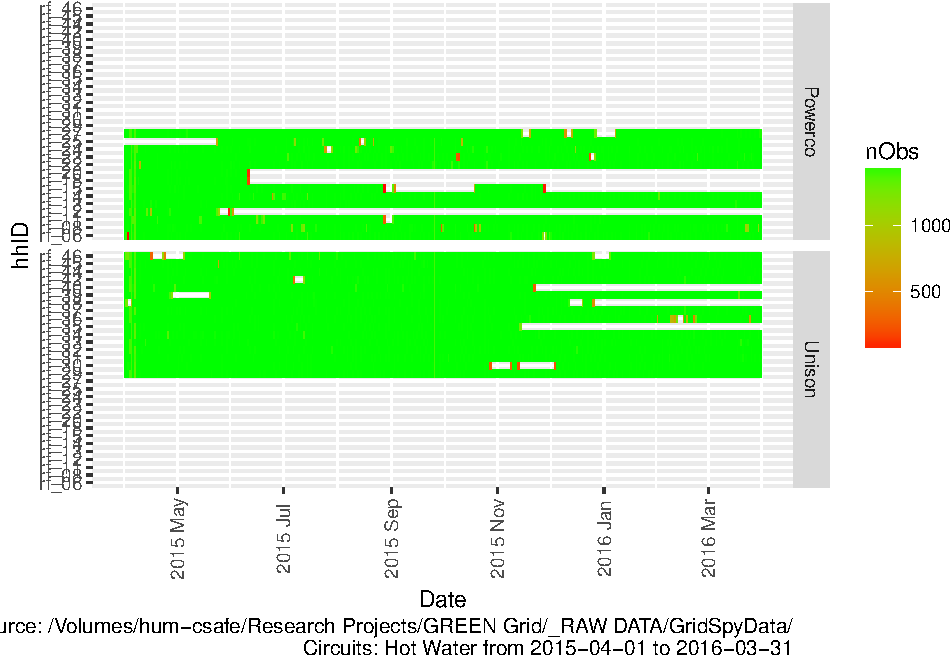
\includegraphics{nzGGHouseholdPowerDemandProfile_Hot Water_2015-04-01_2016-03-31_files/figure-latex/loadedFilesObs Tile Plot-1.pdf}

The next plot shows the same data but as a dot plot to highlight those
households and dates where we did not receive 60 * 24 = 1440
observations per day.

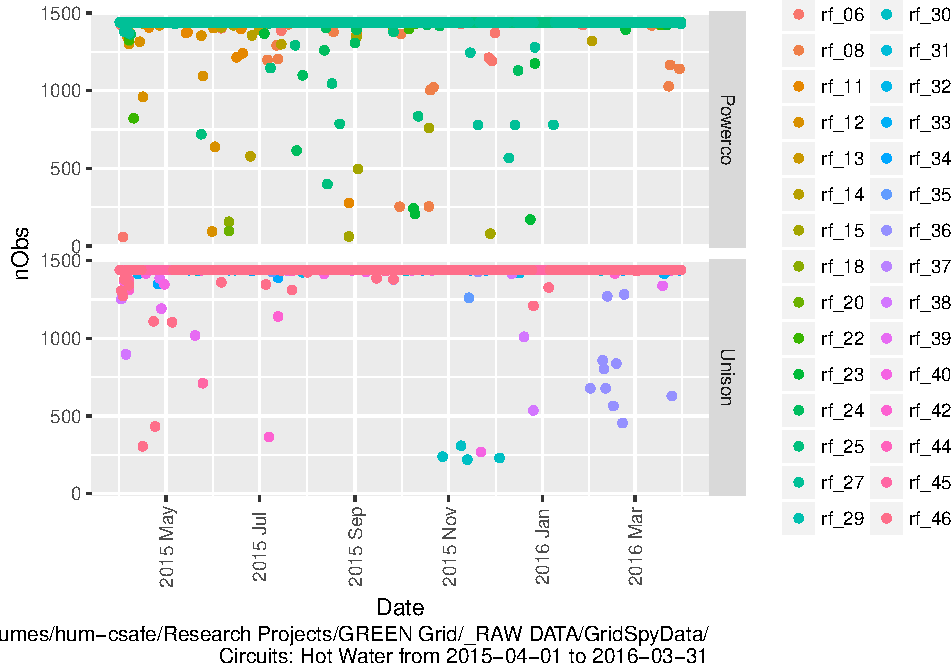
\includegraphics{nzGGHouseholdPowerDemandProfile_Hot Water_2015-04-01_2016-03-31_files/figure-latex/loadedFilesObs point plot-1.pdf}

The following table shows the min/max observations per day and min/max
dates for each household. As above, we should not see:

\begin{itemize}
\tightlist
\item
  dates before 2014 or in to the future (indicates date conversion
  errors)
\item
  more than 1440 observations per day (indicates potentially duplicate
  observations)
\item
  non-integer counts of circuits as it suggests some column errors
\end{itemize}

We should also not see NA in any row (indicates date conversion errors).

If we do see any of these then we still have data cleaning work to do!

\begin{longtable}[]{@{}llrll@{}}
\toprule
hhID & sample & nObs & minDate & maxDate\tabularnewline
\midrule
\endhead
rf\_12 & Powerco & 80021 & 2015-04-01 00:00:00 & 2015-06-02
20:07:00\tabularnewline
rf\_20 & Powerco & 102139 & 2015-04-01 00:00:00 & 2015-06-11
01:37:00\tabularnewline
rf\_18 & Powerco & 102153 & 2015-04-01 00:00:00 & 2015-06-11
02:36:00\tabularnewline
rf\_35 & Unison & 327862 & 2015-04-01 00:00:00 & 2015-11-14
21:00:00\tabularnewline
rf\_40 & Unison & 338208 & 2015-04-01 00:00:00 & 2015-11-22
04:27:00\tabularnewline
rf\_15 & Powerco & 273202 & 2015-04-01 00:00:00 & 2015-11-28
01:19:00\tabularnewline
rf\_38 & Unison & 747324 & 2015-04-01 00:00:00 & 2015-12-26
08:55:00\tabularnewline
rf\_06 & Powerco & 523192 & 2015-04-01 00:00:00 & 2016-03-31
23:59:00\tabularnewline
rf\_08 & Powerco & 521771 & 2015-04-01 00:00:00 & 2016-03-31
23:59:00\tabularnewline
rf\_11 & Powerco & 519082 & 2015-04-01 00:00:00 & 2016-03-31
23:59:00\tabularnewline
rf\_13 & Powerco & 526848 & 2015-04-01 00:00:00 & 2016-03-31
23:59:00\tabularnewline
rf\_14 & Powerco & 525400 & 2015-04-01 00:00:00 & 2016-03-31
23:59:00\tabularnewline
rf\_22 & Powerco & 526015 & 2015-04-01 00:00:00 & 2016-03-31
23:59:00\tabularnewline
rf\_23 & Powerco & 519808 & 2015-04-01 00:00:00 & 2016-03-31
23:59:00\tabularnewline
rf\_24 & Powerco & 520436 & 2015-04-01 00:00:00 & 2016-03-31
23:59:00\tabularnewline
rf\_25 & Powerco & 443882 & 2015-05-24 12:00:00 & 2016-03-31
23:59:00\tabularnewline
rf\_27 & Powerco & 497686 & 2015-04-01 00:00:00 & 2016-03-31
23:59:00\tabularnewline
rf\_29 & Unison & 526661 & 2015-04-01 00:00:00 & 2016-03-31
23:59:00\tabularnewline
rf\_30 & Unison & 477431 & 2015-04-01 00:00:00 & 2016-03-31
23:59:00\tabularnewline
rf\_31 & Unison & 526781 & 2015-04-01 00:00:00 & 2016-03-31
23:59:00\tabularnewline
rf\_32 & Unison & 526680 & 2015-04-01 00:00:00 & 2016-03-31
23:59:00\tabularnewline
rf\_33 & Unison & 526771 & 2015-04-01 00:00:00 & 2016-03-31
23:59:00\tabularnewline
rf\_34 & Unison & 526566 & 2015-04-01 00:00:00 & 2016-03-31
23:59:00\tabularnewline
rf\_36 & Unison & 516142 & 2015-04-01 00:00:00 & 2016-03-31
23:59:00\tabularnewline
rf\_37 & Unison & 526651 & 2015-04-01 00:00:00 & 2016-03-31
23:59:00\tabularnewline
rf\_39 & Unison & 495697 & 2015-04-01 00:00:00 & 2016-03-31
23:59:00\tabularnewline
rf\_42 & Unison & 518074 & 2015-04-01 00:00:00 & 2016-03-31
23:59:00\tabularnewline
rf\_44 & Unison & 526749 & 2015-04-01 00:00:00 & 2016-03-31
23:59:00\tabularnewline
rf\_45 & Unison & 526010 & 2015-04-01 00:00:00 & 2016-03-31
23:59:00\tabularnewline
rf\_46 & Unison & 950796 & 2015-04-01 00:00:00 & 2016-03-31
23:59:00\tabularnewline
\bottomrule
\end{longtable}

Finally we show the total number of households which we think we have
Hot Water data for.

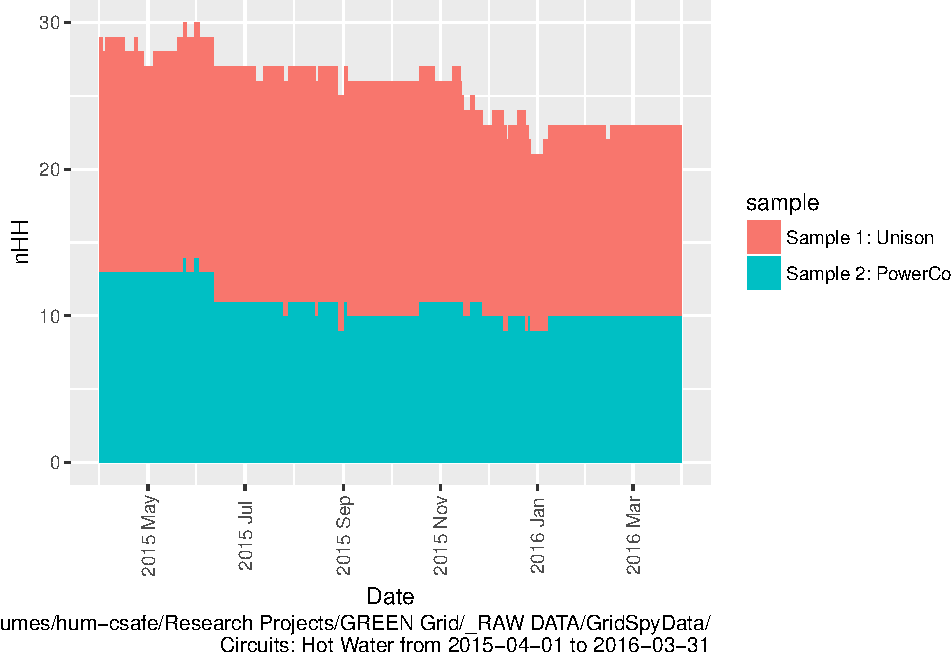
\includegraphics{nzGGHouseholdPowerDemandProfile_Hot Water_2015-04-01_2016-03-31_files/figure-latex/liveDataHouseholds-1.pdf}

The following table summarises the Hot Water data. Any surprises?

\begin{Shaded}
\begin{Highlighting}[]
\NormalTok{t <-}\StringTok{ }\KeywordTok{summary}\NormalTok{(gs1MinDT)}
\NormalTok{knitr}\OperatorTok{::}\KeywordTok{kable}\NormalTok{(}\DataTypeTok{caption =} \KeywordTok{paste0}\NormalTok{(}\StringTok{"Summary of "}\NormalTok{, circuitPattern, }\StringTok{" circuits"}\NormalTok{), t)}
\end{Highlighting}
\end{Shaded}

\begin{longtable}[]{@{}llllll@{}}
\toprule
\begin{minipage}[b]{0.03\columnwidth}\raggedright\strut
\strut
\end{minipage} & \begin{minipage}[b]{0.15\columnwidth}\raggedright\strut
hhID\strut
\end{minipage} & \begin{minipage}[b]{0.24\columnwidth}\raggedright\strut
r\_dateTime\strut
\end{minipage} & \begin{minipage}[b]{0.15\columnwidth}\raggedright\strut
circuitLabel\strut
\end{minipage} & \begin{minipage}[b]{0.12\columnwidth}\raggedright\strut
circuitID\strut
\end{minipage} & \begin{minipage}[b]{0.14\columnwidth}\raggedright\strut
powerW\strut
\end{minipage}\tabularnewline
\midrule
\endhead
\begin{minipage}[t]{0.03\columnwidth}\raggedright\strut
\strut
\end{minipage} & \begin{minipage}[t]{0.15\columnwidth}\raggedright\strut
Length:14493877\strut
\end{minipage} & \begin{minipage}[t]{0.24\columnwidth}\raggedright\strut
Min. :2015-04-01 00:00:00\strut
\end{minipage} & \begin{minipage}[t]{0.15\columnwidth}\raggedright\strut
Length:14493877\strut
\end{minipage} & \begin{minipage}[t]{0.12\columnwidth}\raggedright\strut
Min. :1574\strut
\end{minipage} & \begin{minipage}[t]{0.14\columnwidth}\raggedright\strut
Min. :-1110.0\strut
\end{minipage}\tabularnewline
\begin{minipage}[t]{0.03\columnwidth}\raggedright\strut
\strut
\end{minipage} & \begin{minipage}[t]{0.15\columnwidth}\raggedright\strut
Class :character\strut
\end{minipage} & \begin{minipage}[t]{0.24\columnwidth}\raggedright\strut
1st Qu.:2015-06-22 16:46:00\strut
\end{minipage} & \begin{minipage}[t]{0.15\columnwidth}\raggedright\strut
Class :character\strut
\end{minipage} & \begin{minipage}[t]{0.12\columnwidth}\raggedright\strut
1st Qu.:2248\strut
\end{minipage} & \begin{minipage}[t]{0.14\columnwidth}\raggedright\strut
1st Qu.: 0.0\strut
\end{minipage}\tabularnewline
\begin{minipage}[t]{0.03\columnwidth}\raggedright\strut
\strut
\end{minipage} & \begin{minipage}[t]{0.15\columnwidth}\raggedright\strut
Mode :character\strut
\end{minipage} & \begin{minipage}[t]{0.24\columnwidth}\raggedright\strut
Median :2015-09-18 21:32:00\strut
\end{minipage} & \begin{minipage}[t]{0.15\columnwidth}\raggedright\strut
Mode :character\strut
\end{minipage} & \begin{minipage}[t]{0.12\columnwidth}\raggedright\strut
Median :4135\strut
\end{minipage} & \begin{minipage}[t]{0.14\columnwidth}\raggedright\strut
Median : 0.0\strut
\end{minipage}\tabularnewline
\begin{minipage}[t]{0.03\columnwidth}\raggedright\strut
\strut
\end{minipage} & \begin{minipage}[t]{0.15\columnwidth}\raggedright\strut
NA\strut
\end{minipage} & \begin{minipage}[t]{0.24\columnwidth}\raggedright\strut
Mean :2015-09-22 19:59:55\strut
\end{minipage} & \begin{minipage}[t]{0.15\columnwidth}\raggedright\strut
NA\strut
\end{minipage} & \begin{minipage}[t]{0.12\columnwidth}\raggedright\strut
Mean :3421\strut
\end{minipage} & \begin{minipage}[t]{0.14\columnwidth}\raggedright\strut
Mean : 283.8\strut
\end{minipage}\tabularnewline
\begin{minipage}[t]{0.03\columnwidth}\raggedright\strut
\strut
\end{minipage} & \begin{minipage}[t]{0.15\columnwidth}\raggedright\strut
NA\strut
\end{minipage} & \begin{minipage}[t]{0.24\columnwidth}\raggedright\strut
3rd Qu.:2015-12-20 17:19:00\strut
\end{minipage} & \begin{minipage}[t]{0.15\columnwidth}\raggedright\strut
NA\strut
\end{minipage} & \begin{minipage}[t]{0.12\columnwidth}\raggedright\strut
3rd Qu.:4184\strut
\end{minipage} & \begin{minipage}[t]{0.14\columnwidth}\raggedright\strut
3rd Qu.: 0.0\strut
\end{minipage}\tabularnewline
\begin{minipage}[t]{0.03\columnwidth}\raggedright\strut
\strut
\end{minipage} & \begin{minipage}[t]{0.15\columnwidth}\raggedright\strut
NA\strut
\end{minipage} & \begin{minipage}[t]{0.24\columnwidth}\raggedright\strut
Max. :2016-03-31 23:59:00\strut
\end{minipage} & \begin{minipage}[t]{0.15\columnwidth}\raggedright\strut
NA\strut
\end{minipage} & \begin{minipage}[t]{0.12\columnwidth}\raggedright\strut
Max. :4400\strut
\end{minipage} & \begin{minipage}[t]{0.14\columnwidth}\raggedright\strut
Max. : 4076.0\strut
\end{minipage}\tabularnewline
\bottomrule
\end{longtable}

We seem to have some negative powerW values and at least one very large
power value.

Nasty surprises often lurk in histograms\ldots{} The following histogram
shows all observations.

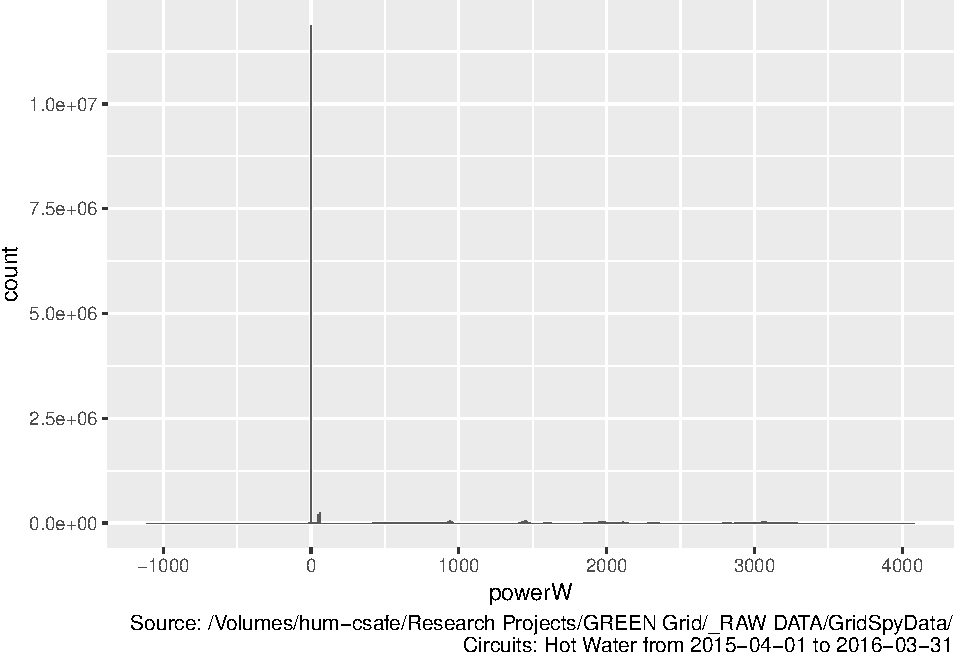
\includegraphics{nzGGHouseholdPowerDemandProfile_Hot Water_2015-04-01_2016-03-31_files/figure-latex/histo full-1.pdf}

The next shows the histogram for powerW \textless{} 1000W\ldots{}

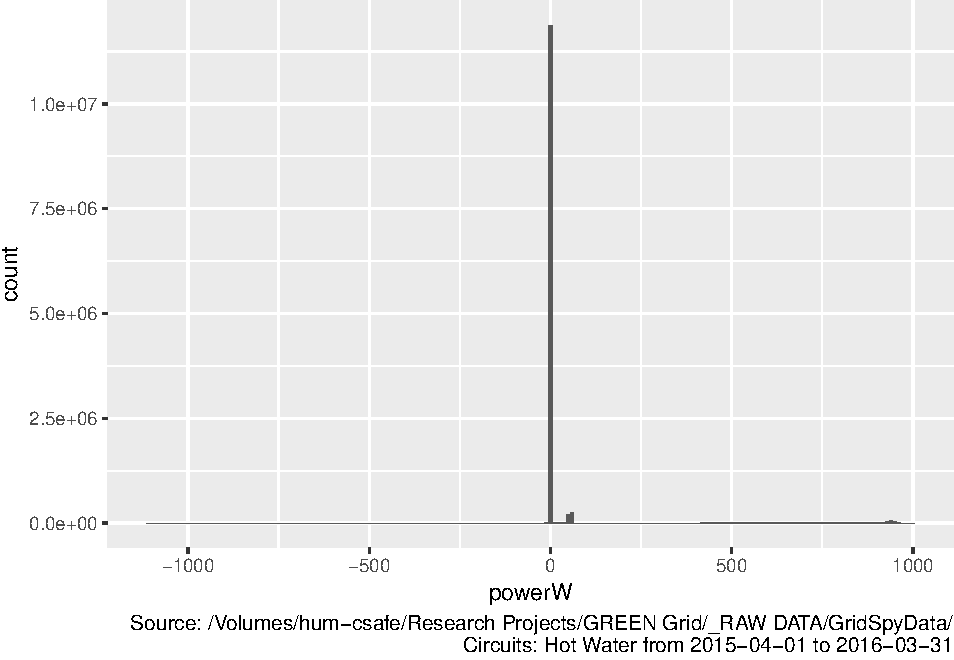
\includegraphics{nzGGHouseholdPowerDemandProfile_Hot Water_2015-04-01_2016-03-31_files/figure-latex/histo power under 1000-1.pdf}

\begin{quote}
There are a lot of zeros (as we'd expect) but why are there negative
values?
\end{quote}

\section{Hot Water profiles}\label{hot-water-profiles}

This section produces the profiles as one for each HH but averaged over
each season. Data is kept at 1 minute intervals. Note definition of
season below\ldots{}

\begin{Shaded}
\begin{Highlighting}[]
\CommentTok{# add season}
\NormalTok{gs1MinDT <-}\StringTok{ }\NormalTok{gs1MinDT[, month }\OperatorTok{:}\ErrorTok{=}\StringTok{ }\NormalTok{lubridate}\OperatorTok{::}\KeywordTok{month}\NormalTok{(r_dateTime, }\DataTypeTok{label =} \OtherTok{TRUE}\NormalTok{)]}
\NormalTok{gs1MinDT <-}\StringTok{ }\NormalTok{gs1MinDT[, season }\OperatorTok{:}\ErrorTok{=}\StringTok{ "Summer"}\NormalTok{]}
\NormalTok{gs1MinDT <-}\StringTok{ }\NormalTok{gs1MinDT[, season }\OperatorTok{:}\ErrorTok{=}\StringTok{ }\KeywordTok{ifelse}\NormalTok{(month }\OperatorTok{==}\StringTok{ "Mar"} \OperatorTok{|}
\StringTok{                                              }\NormalTok{month }\OperatorTok{==}\StringTok{ "Apr"} \OperatorTok{|}
\StringTok{                                              }\NormalTok{month }\OperatorTok{==}\StringTok{ "May"}\NormalTok{, }\StringTok{"Autumn"}\NormalTok{, season)]}
\NormalTok{gs1MinDT <-}\StringTok{ }\NormalTok{gs1MinDT[, season }\OperatorTok{:}\ErrorTok{=}\StringTok{ }\KeywordTok{ifelse}\NormalTok{(month }\OperatorTok{==}\StringTok{ "Jun"} \OperatorTok{|}
\StringTok{                                              }\NormalTok{month }\OperatorTok{==}\StringTok{ "Jul"} \OperatorTok{|}
\StringTok{                                              }\NormalTok{month }\OperatorTok{==}\StringTok{ "Aug"}\NormalTok{, }\StringTok{"Winter"}\NormalTok{, season)]}
\NormalTok{gs1MinDT <-}\StringTok{ }\NormalTok{gs1MinDT[, season }\OperatorTok{:}\ErrorTok{=}\StringTok{ }\KeywordTok{ifelse}\NormalTok{(month }\OperatorTok{==}\StringTok{ "Sep"} \OperatorTok{|}
\StringTok{                                              }\NormalTok{month }\OperatorTok{==}\StringTok{ "Oct"} \OperatorTok{|}
\StringTok{                                              }\NormalTok{month }\OperatorTok{==}\StringTok{ "Nov"}\NormalTok{, }\StringTok{"Spring"}\NormalTok{, season)]}
\end{Highlighting}
\end{Shaded}

\subsection{Profile plots: means per
household}\label{profile-plots-means-per-household}

This section shows a plot of mean profiles for each household by season.

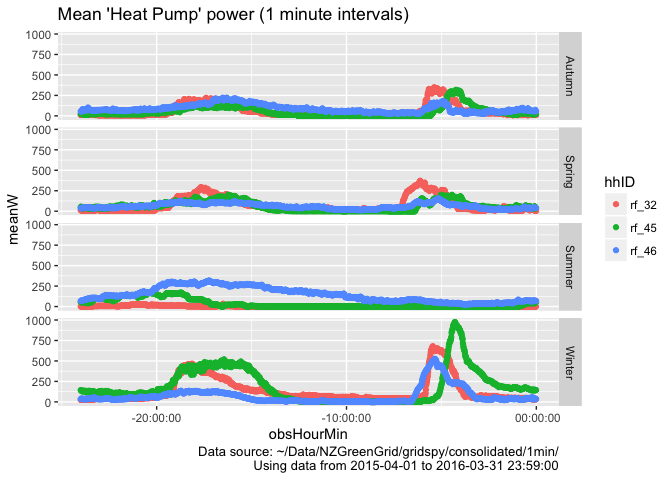
\includegraphics{nzGGHouseholdPowerDemandProfile_Hot Water_2015-04-01_2016-03-31_files/figure-latex/profiles per household by season-1.pdf}

\begin{verbatim}
## [1] "Saving plot to /Volumes/hum-csafe/Research Projects/GREEN Grid/Clean_data/safe/gridSpy/1min/profiles/Hot Water_2015-04-01_2016-03-31_byHouseholdSeasonalProfilePlot.pdf"
\end{verbatim}

\begin{verbatim}
## [1] "Saving profile data used to build this plot to: /Volumes/hum-csafe/Research Projects/GREEN Grid/Clean_data/safe/gridSpy/1min/profiles/Hot Water_2015-04-01_2016-03-31_byHouseholdSeasonalProfiles.csv..."
\end{verbatim}

\begin{verbatim}
## [1] "Gzipped /Volumes/hum-csafe/Research Projects/GREEN Grid/Clean_data/safe/gridSpy/1min/profiles/Hot Water_2015-04-01_2016-03-31_byHouseholdSeasonalProfiles.csv"
\end{verbatim}

\begin{longtable}[]{@{}lllll@{}}
\toprule
& hhID & obsHourMin & season & meanW\tabularnewline
\midrule
\endhead
& Length:167011 & Length:167011 & Length:167011 & Min. :
-8.279\tabularnewline
& Class :character & Class1:hms & Class :character & 1st Qu.:
69.255\tabularnewline
& Mode :character & Class2:difftime & Mode :character & Median :
193.417\tabularnewline
& NA & Mode :numeric & NA & Mean : 293.940\tabularnewline
& NA & NA & NA & 3rd Qu.: 389.015\tabularnewline
& NA & NA & NA & Max. :3072.650\tabularnewline
\bottomrule
\end{longtable}

As we can see there is considerable variation between households in both
the level and timing of heat pump demand.

Note that the code saves a high definition version of the plot and the
profiles for future re-use.

The .csv.gz file can be loaded using the following code:

\begin{itemize}
\tightlist
\item
  \texttt{df\ \textless{}-\ readr::read\_csv("/Volumes/hum-csafe/Research\ Projects/GREEN\ Grid/Clean\_data/safe/gridSpy/1min/profiles/Hot\ Water\_2015-04-01\_2016-03-31\_byHouseholdSeasonalProfiles.csv.gz")}
  or
\item
  \texttt{dt\ \textless{}-\ data.table::as.data.table(readr::read\_csv("/Volumes/hum-csafe/Research\ Projects/GREEN\ Grid/Clean\_data/safe/gridSpy/1min/profiles/Hot\ Water\_2015-04-01\_2016-03-31\_byHouseholdSeasonalProfiles.csv.gz"))}
  if you prefer \texttt{data.table}
\end{itemize}

\subsection{Profile plots: overall household
mean}\label{profile-plots-overall-household-mean}

This section shows a plot of mean and median profiles across all
household by season. The mean profile also shows the level of variance
by plotting error bars at +/- 1 s.d.

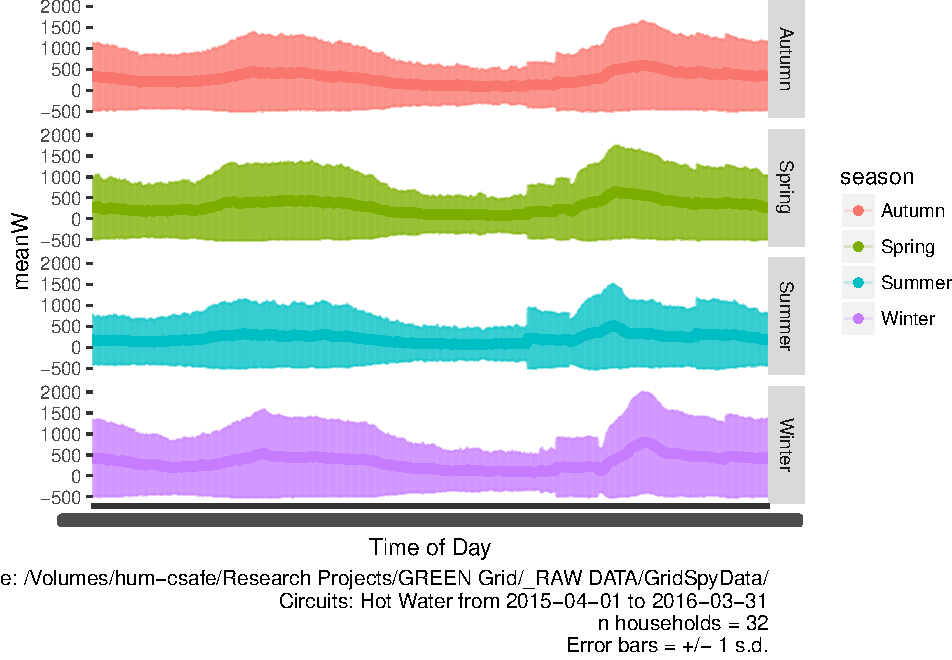
\includegraphics{nzGGHouseholdPowerDemandProfile_Hot Water_2015-04-01_2016-03-31_files/figure-latex/overall profiles by season-1.pdf}

\begin{verbatim}
## [1] "Saving plot to /Volumes/hum-csafe/Research Projects/GREEN Grid/Clean_data/safe/gridSpy/1min/profiles/Hot Water_2015-04-01_2016-03-31_overallMeanSeasonalProfilePlot.pdf"
\end{verbatim}

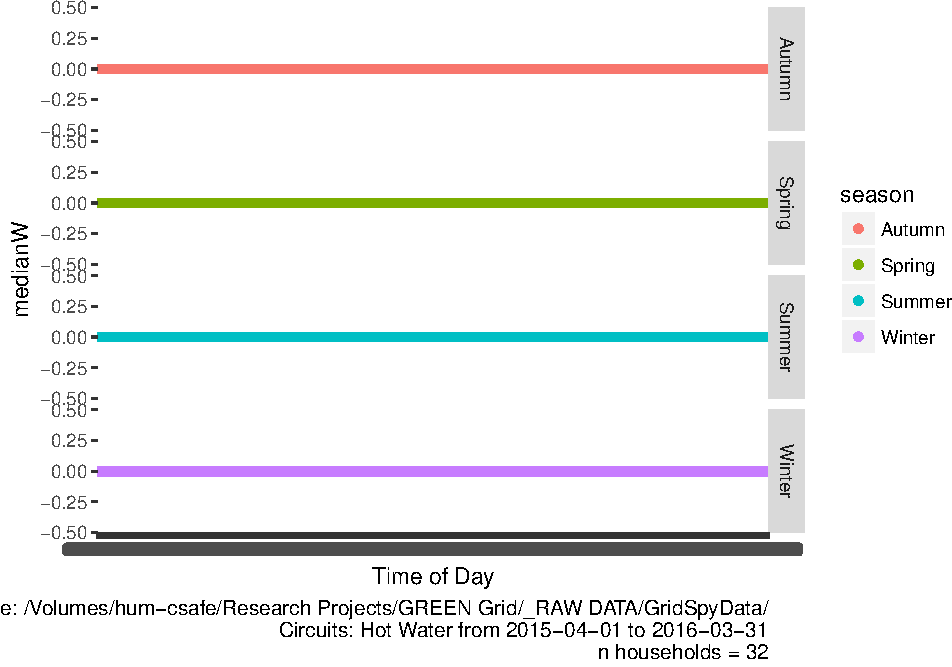
\includegraphics{nzGGHouseholdPowerDemandProfile_Hot Water_2015-04-01_2016-03-31_files/figure-latex/overall profiles by season-2.pdf}

\begin{verbatim}
## [1] "Saving plot to /Volumes/hum-csafe/Research Projects/GREEN Grid/Clean_data/safe/gridSpy/1min/profiles/Hot Water_2015-04-01_2016-03-31_overallMedianSeasonalProfilePlot.pdf"
\end{verbatim}

\begin{verbatim}
## [1] "Saving profile data used to build this plot to: /Volumes/hum-csafe/Research Projects/GREEN Grid/Clean_data/safe/gridSpy/1min/profiles/Hot Water_2015-04-01_2016-03-31_overallSeasonalProfiles.csv..."
\end{verbatim}

\begin{verbatim}
## [1] "Gzipped /Volumes/hum-csafe/Research Projects/GREEN Grid/Clean_data/safe/gridSpy/1min/profiles/Hot Water_2015-04-01_2016-03-31_overallSeasonalProfiles.csv"
\end{verbatim}

\begin{longtable}[]{@{}lllllll@{}}
\toprule
\begin{minipage}[b]{0.03\columnwidth}\raggedright\strut
\strut
\end{minipage} & \begin{minipage}[b]{0.14\columnwidth}\raggedright\strut
obsHourMin\strut
\end{minipage} & \begin{minipage}[b]{0.15\columnwidth}\raggedright\strut
season\strut
\end{minipage} & \begin{minipage}[b]{0.13\columnwidth}\raggedright\strut
meanW\strut
\end{minipage} & \begin{minipage}[b]{0.10\columnwidth}\raggedright\strut
medianW\strut
\end{minipage} & \begin{minipage}[b]{0.12\columnwidth}\raggedright\strut
nObs\strut
\end{minipage} & \begin{minipage}[b]{0.13\columnwidth}\raggedright\strut
sdW\strut
\end{minipage}\tabularnewline
\midrule
\endhead
\begin{minipage}[t]{0.03\columnwidth}\raggedright\strut
\strut
\end{minipage} & \begin{minipage}[t]{0.14\columnwidth}\raggedright\strut
Length:5760\strut
\end{minipage} & \begin{minipage}[t]{0.15\columnwidth}\raggedright\strut
Length:5760\strut
\end{minipage} & \begin{minipage}[t]{0.13\columnwidth}\raggedright\strut
Min. : 58.62\strut
\end{minipage} & \begin{minipage}[t]{0.10\columnwidth}\raggedright\strut
Min. :0\strut
\end{minipage} & \begin{minipage}[t]{0.12\columnwidth}\raggedright\strut
Min. :2230\strut
\end{minipage} & \begin{minipage}[t]{0.13\columnwidth}\raggedright\strut
Min. : 320.4\strut
\end{minipage}\tabularnewline
\begin{minipage}[t]{0.03\columnwidth}\raggedright\strut
\strut
\end{minipage} & \begin{minipage}[t]{0.14\columnwidth}\raggedright\strut
Class1:hms\strut
\end{minipage} & \begin{minipage}[t]{0.15\columnwidth}\raggedright\strut
Class :character\strut
\end{minipage} & \begin{minipage}[t]{0.13\columnwidth}\raggedright\strut
1st Qu.:170.19\strut
\end{minipage} & \begin{minipage}[t]{0.10\columnwidth}\raggedright\strut
1st Qu.:0\strut
\end{minipage} & \begin{minipage}[t]{0.12\columnwidth}\raggedright\strut
1st Qu.:2430\strut
\end{minipage} & \begin{minipage}[t]{0.13\columnwidth}\raggedright\strut
1st Qu.: 576.9\strut
\end{minipage}\tabularnewline
\begin{minipage}[t]{0.03\columnwidth}\raggedright\strut
\strut
\end{minipage} & \begin{minipage}[t]{0.14\columnwidth}\raggedright\strut
Class2:difftime\strut
\end{minipage} & \begin{minipage}[t]{0.15\columnwidth}\raggedright\strut
Mode :character\strut
\end{minipage} & \begin{minipage}[t]{0.13\columnwidth}\raggedright\strut
Median :261.01\strut
\end{minipage} & \begin{minipage}[t]{0.10\columnwidth}\raggedright\strut
Median :0\strut
\end{minipage} & \begin{minipage}[t]{0.12\columnwidth}\raggedright\strut
Median :2569\strut
\end{minipage} & \begin{minipage}[t]{0.13\columnwidth}\raggedright\strut
Median : 725.2\strut
\end{minipage}\tabularnewline
\begin{minipage}[t]{0.03\columnwidth}\raggedright\strut
\strut
\end{minipage} & \begin{minipage}[t]{0.14\columnwidth}\raggedright\strut
Mode :numeric\strut
\end{minipage} & \begin{minipage}[t]{0.15\columnwidth}\raggedright\strut
NA\strut
\end{minipage} & \begin{minipage}[t]{0.13\columnwidth}\raggedright\strut
Mean :281.21\strut
\end{minipage} & \begin{minipage}[t]{0.10\columnwidth}\raggedright\strut
Mean :0\strut
\end{minipage} & \begin{minipage}[t]{0.12\columnwidth}\raggedright\strut
Mean :2516\strut
\end{minipage} & \begin{minipage}[t]{0.13\columnwidth}\raggedright\strut
Mean : 721.3\strut
\end{minipage}\tabularnewline
\begin{minipage}[t]{0.03\columnwidth}\raggedright\strut
\strut
\end{minipage} & \begin{minipage}[t]{0.14\columnwidth}\raggedright\strut
NA\strut
\end{minipage} & \begin{minipage}[t]{0.15\columnwidth}\raggedright\strut
NA\strut
\end{minipage} & \begin{minipage}[t]{0.13\columnwidth}\raggedright\strut
3rd Qu.:386.90\strut
\end{minipage} & \begin{minipage}[t]{0.10\columnwidth}\raggedright\strut
3rd Qu.:0\strut
\end{minipage} & \begin{minipage}[t]{0.12\columnwidth}\raggedright\strut
3rd Qu.:2657\strut
\end{minipage} & \begin{minipage}[t]{0.13\columnwidth}\raggedright\strut
3rd Qu.: 876.0\strut
\end{minipage}\tabularnewline
\begin{minipage}[t]{0.03\columnwidth}\raggedright\strut
\strut
\end{minipage} & \begin{minipage}[t]{0.14\columnwidth}\raggedright\strut
NA\strut
\end{minipage} & \begin{minipage}[t]{0.15\columnwidth}\raggedright\strut
NA\strut
\end{minipage} & \begin{minipage}[t]{0.13\columnwidth}\raggedright\strut
Max. :805.88\strut
\end{minipage} & \begin{minipage}[t]{0.10\columnwidth}\raggedright\strut
Max. :0\strut
\end{minipage} & \begin{minipage}[t]{0.12\columnwidth}\raggedright\strut
Max. :2671\strut
\end{minipage} & \begin{minipage}[t]{0.13\columnwidth}\raggedright\strut
Max. :1208.5\strut
\end{minipage}\tabularnewline
\bottomrule
\end{longtable}

The difference between the mean and median plots is instructive - it
suggests that the mean plots for summer are skewed by a few higher heat
pump-using households.

The plots could be repeated or re-facted e.g.~by household size.

As before, the code saves a high definition version of the plot and the
profiles for future re-use.

\section{Runtime}\label{runtime}

Analysis completed in 130.32 seconds ( 2.17 minutes) using
\href{https://cran.r-project.org/package=knitr}{knitr} in
\href{http://www.rstudio.com}{RStudio} with R version 3.5.0 (2018-04-23)
running on x86\_64-apple-darwin15.6.0.

\section{R environment}\label{r-environment}

R packages used:

\begin{itemize}
\tightlist
\item
  base R - for the basics (R Core Team 2016)
\item
  data.table - for fast (big) data handling (Dowle et al. 2015)
\item
  lubridate - date manipulation (Grolemund and Wickham 2011)
\item
  ggplot2 - for slick graphics (Wickham 2009)
\item
  readr - for csv reading/writing (Wickham, Hester, and Francois 2016)
\item
  dplyr - for select and contains (Wickham and Francois 2016)
\item
  progress - for progress bars (Csárdi and FitzJohn 2016)
\item
  knitr - to create this document \& neat tables (Xie 2016)
\item
  nzGREENGrid - for local NZ GREEN Grid project utilities
\end{itemize}

Session info:

\begin{verbatim}
## R version 3.5.0 (2018-04-23)
## Platform: x86_64-apple-darwin15.6.0 (64-bit)
## Running under: macOS High Sierra 10.13.6
## 
## Matrix products: default
## BLAS: /System/Library/Frameworks/Accelerate.framework/Versions/A/Frameworks/vecLib.framework/Versions/A/libBLAS.dylib
## LAPACK: /Library/Frameworks/R.framework/Versions/3.5/Resources/lib/libRlapack.dylib
## 
## locale:
## [1] en_GB.UTF-8/en_GB.UTF-8/en_GB.UTF-8/C/en_GB.UTF-8/en_GB.UTF-8
## 
## attached base packages:
## [1] stats     graphics  grDevices utils     datasets  methods   base     
## 
## other attached packages:
## [1] kableExtra_0.9.0  knitr_1.20        readr_1.1.1       ggplot2_2.2.1    
## [5] dplyr_0.7.5       data.table_1.11.4 rmarkdown_1.10    nzGREENGrid_0.1.0
## 
## loaded via a namespace (and not attached):
##  [1] tinytex_0.5       tidyselect_0.2.4  reshape2_1.4.3   
##  [4] purrr_0.2.5       lattice_0.20-35   colorspace_1.3-2 
##  [7] htmltools_0.3.6   viridisLite_0.3.0 yaml_2.1.19      
## [10] utf8_1.1.4        rlang_0.2.1       pillar_1.2.3     
## [13] glue_1.2.0        sp_1.3-1          readxl_1.1.0     
## [16] bindrcpp_0.2.2    jpeg_0.1-8        bindr_0.1.1      
## [19] plyr_1.8.4        stringr_1.3.1     cellranger_1.1.0 
## [22] munsell_0.5.0     gtable_0.2.0      rvest_0.3.2      
## [25] RgoogleMaps_1.4.2 mapproj_1.2.6     evaluate_0.10.1  
## [28] labeling_0.3      highr_0.7         proto_1.0.0      
## [31] Rcpp_0.12.17      geosphere_1.5-7   openssl_1.0.1    
## [34] scales_0.5.0      backports_1.1.2   rjson_0.2.20     
## [37] hms_0.4.2         png_0.1-7         digest_0.6.15    
## [40] stringi_1.2.3     grid_3.5.0        rprojroot_1.3-2  
## [43] cli_1.0.0         tools_3.5.0       magrittr_1.5     
## [46] maps_3.3.0        lazyeval_0.2.1    tibble_1.4.2     
## [49] crayon_1.3.4      pkgconfig_2.0.1   xml2_1.2.0       
## [52] lubridate_1.7.4   assertthat_0.2.0  httr_1.3.1       
## [55] rstudioapi_0.7    R6_2.2.2          ggmap_2.6.1      
## [58] compiler_3.5.0
\end{verbatim}

\section*{References}\label{references}
\addcontentsline{toc}{section}{References}

\hypertarget{refs}{}
\hypertarget{ref-progress}{}
Csárdi, Gábor, and Rich FitzJohn. 2016. \emph{Progress: Terminal
Progress Bars}. \url{https://CRAN.R-project.org/package=progress}.

\hypertarget{ref-data.table}{}
Dowle, M, A Srinivasan, T Short, S Lianoglou with contributions from R
Saporta, and E Antonyan. 2015. \emph{Data.table: Extension of
Data.frame}. \url{https://CRAN.R-project.org/package=data.table}.

\hypertarget{ref-lubridate}{}
Grolemund, Garrett, and Hadley Wickham. 2011. ``Dates and Times Made
Easy with lubridate.'' \emph{Journal of Statistical Software} 40 (3):
1--25. \url{http://www.jstatsoft.org/v40/i03/}.

\hypertarget{ref-baseR}{}
R Core Team. 2016. \emph{R: A Language and Environment for Statistical
Computing}. Vienna, Austria: R Foundation for Statistical Computing.
\url{https://www.R-project.org/}.

\hypertarget{ref-ggplot2}{}
Wickham, Hadley. 2009. \emph{Ggplot2: Elegant Graphics for Data
Analysis}. Springer-Verlag New York. \url{http://ggplot2.org}.

\hypertarget{ref-dplyr}{}
Wickham, Hadley, and Romain Francois. 2016. \emph{Dplyr: A Grammar of
Data Manipulation}. \url{https://CRAN.R-project.org/package=dplyr}.

\hypertarget{ref-readr}{}
Wickham, Hadley, Jim Hester, and Romain Francois. 2016. \emph{Readr:
Read Tabular Data}. \url{https://CRAN.R-project.org/package=readr}.

\hypertarget{ref-knitr}{}
Xie, Yihui. 2016. \emph{Knitr: A General-Purpose Package for Dynamic
Report Generation in R}. \url{https://CRAN.R-project.org/package=knitr}.


\end{document}
